\documentclass[conference]{IEEEtran}
\usepackage{cite}
\usepackage{amsmath,amssymb,amsfonts}
\usepackage{algorithmic}
\usepackage{graphicx}
\usepackage{textcomp}
\usepackage{listings}
\usepackage{hyperref}
\newcommand{\missingNumber}{\textcolor{red}{XX}\xspace}
\newcommand{\missingPercentage}{\textcolor{red}{XX\%}\xspace}
\newcommand{\missingTable}{\textcolor{red}{XXTable}\xspace}
\newcommand{\missingGraph}{\textcolor{red}{XXGraph}\xspace}
\usepackage[usenames,dvipsnames]{xcolor}
\usepackage{paralist}
\usepackage{xspace}
\usepackage{url}

\newcommand{\CoreEvalCallCountRnd}{12.6M\xspace}
\newcommand{\CoreEvalCallCount}{12,637,139\xspace}
\newcommand{\CoreEvalSiteCountRnd}{170\xspace}
\newcommand{\CoreEvalSiteCount}{170\xspace}
\newcommand{\CoreEvalParentCallCountRnd}{254.1K\xspace}
\newcommand{\CoreEvalParentCallCount}{254,112\xspace}
\newcommand{\CoreEvalParentSiteCountRnd}{16\xspace}
\newcommand{\CoreEvalParentSiteCount}{16\xspace}
\newcommand{\CoreEvalqCallCountRnd}{265.5K\xspace}
\newcommand{\CoreEvalqCallCount}{265,499\xspace}
\newcommand{\CoreEvalqSiteCountRnd}{4\xspace}
\newcommand{\CoreEvalqSiteCount}{4\xspace}
\newcommand{\CoreLocalCallCountRnd}{234.2K\xspace}
\newcommand{\CoreLocalCallCount}{234,212\xspace}
\newcommand{\CoreLocalSiteCountRnd}{1.1K\xspace}
\newcommand{\CoreLocalSiteCount}{1,116\xspace}
\newcommand{\PackageEvalCallCountRnd}{5M\xspace}
\newcommand{\PackageEvalCallCount}{5,021,240\xspace}
\newcommand{\PackageEvalSiteCountRnd}{2.4K\xspace}
\newcommand{\PackageEvalSiteCount}{2,448\xspace}
\newcommand{\PackageEvalParentCallCountRnd}{52.1K\xspace}
\newcommand{\PackageEvalParentCallCount}{52,130\xspace}
\newcommand{\PackageEvalParentSiteCountRnd}{351\xspace}
\newcommand{\PackageEvalParentSiteCount}{351\xspace}
\newcommand{\PackageEvalqCallCountRnd}{292\xspace}
\newcommand{\PackageEvalqCallCount}{292\xspace}
\newcommand{\PackageEvalqSiteCountRnd}{7\xspace}
\newcommand{\PackageEvalqSiteCount}{7\xspace}
\newcommand{\PackageLocalCallCountRnd}{1.3K\xspace}
\newcommand{\PackageLocalCallCount}{1,251\xspace}
\newcommand{\PackageLocalSiteCountRnd}{8\xspace}
\newcommand{\PackageLocalSiteCount}{8\xspace}
\newcommand{\KaggleEvalCallCountRnd}{0\xspace}
\newcommand{\KaggleEvalCallCount}{0\xspace}
\newcommand{\KaggleEvalSiteCountRnd}{0\xspace}
\newcommand{\KaggleEvalSiteCount}{0\xspace}
\newcommand{\KaggleEvalParentCallCountRnd}{0\xspace}
\newcommand{\KaggleEvalParentCallCount}{0\xspace}
\newcommand{\KaggleEvalParentSiteCountRnd}{0\xspace}
\newcommand{\KaggleEvalParentSiteCount}{0\xspace}
\newcommand{\KaggleEvalqCallCountRnd}{0\xspace}
\newcommand{\KaggleEvalqCallCount}{0\xspace}
\newcommand{\KaggleEvalqSiteCountRnd}{0\xspace}
\newcommand{\KaggleEvalqSiteCount}{0\xspace}
\newcommand{\KaggleLocalCallCountRnd}{0\xspace}
\newcommand{\KaggleLocalCallCount}{0\xspace}
\newcommand{\KaggleLocalSiteCountRnd}{0\xspace}
\newcommand{\KaggleLocalSiteCount}{0\xspace}
\newcommand{\CoreAllCallCountRnd}{13.4M\xspace}
\newcommand{\CoreAllCallCount}{13,390,962\xspace}
\newcommand{\CoreAllSiteCountRnd}{1.3K\xspace}
\newcommand{\CoreAllSiteCount}{1,306\xspace}
\newcommand{\KaggleAllCallCountRnd}{0\xspace}
\newcommand{\KaggleAllCallCount}{0\xspace}
\newcommand{\KaggleAllSiteCountRnd}{0\xspace}
\newcommand{\KaggleAllSiteCount}{0\xspace}
\newcommand{\PackageAllCallCountRnd}{5.1M\xspace}
\newcommand{\PackageAllCallCount}{5,074,913\xspace}
\newcommand{\PackageAllSiteCountRnd}{2.8K\xspace}
\newcommand{\PackageAllSiteCount}{2,814\xspace}
\newcommand{\AllEvalCallCountRnd}{17.7M\xspace}
\newcommand{\AllEvalCallCount}{17,658,379\xspace}
\newcommand{\AllEvalSiteCountRnd}{2.6K\xspace}
\newcommand{\AllEvalSiteCount}{2,618\xspace}
\newcommand{\AllEvalParentCallCountRnd}{306.2K\xspace}
\newcommand{\AllEvalParentCallCount}{306,242\xspace}
\newcommand{\AllEvalParentSiteCountRnd}{367\xspace}
\newcommand{\AllEvalParentSiteCount}{367\xspace}
\newcommand{\AllEvalqCallCountRnd}{265.8K\xspace}
\newcommand{\AllEvalqCallCount}{265,791\xspace}
\newcommand{\AllEvalqSiteCountRnd}{11\xspace}
\newcommand{\AllEvalqSiteCount}{11\xspace}
\newcommand{\AllLocalCallCountRnd}{235.5K\xspace}
\newcommand{\AllLocalCallCount}{235,463\xspace}
\newcommand{\AllLocalSiteCountRnd}{1.1K\xspace}
\newcommand{\AllLocalSiteCount}{1,124\xspace}
\newcommand{\AllAllCallCountRnd}{18.5M\xspace}
\newcommand{\AllAllCallCount}{18,465,875\xspace}
\newcommand{\AllAllSiteCountRnd}{4.1K\xspace}
\newcommand{\AllAllSiteCount}{4,120\xspace}
\newcommand{\TotalFileCountRnd}{23.9K\xspace}
\newcommand{\TotalFileCount}{23,871\xspace}
\newcommand{\NoEvalFileCountRnd}{0\xspace}
\newcommand{\NoEvalFileCount}{0\xspace}
\newcommand{\NoEvalFilePerc}{0\%\xspace}
\newcommand{\CoreEvalFileCountRnd}{13.6K\xspace}
\newcommand{\CoreEvalFileCount}{13,584\xspace}
\newcommand{\CoreEvalFilePerc}{56.9\%\xspace}
\newcommand{\PackageEvalFileCountRnd}{224\xspace}
\newcommand{\PackageEvalFileCount}{224\xspace}
\newcommand{\PackageEvalFilePerc}{0.9\%\xspace}
\newcommand{\AllEvalFileCountRnd}{10.1K\xspace}
\newcommand{\AllEvalFileCount}{10,063\xspace}
\newcommand{\AllEvalFilePerc}{42.2\%\xspace}
\newcommand{\EightyCoreEvalFileCountRnd}{5.9K\xspace}
\newcommand{\EightyCoreEvalFileCount}{5,930\xspace}
\newcommand{\EightyCoreEvalFilePerc}{58.9\%\xspace}
\newcommand{\TopTenPackageCallCountRnd}{3.8M\xspace}
\newcommand{\TopTenPackageCallCount}{3,794,346\xspace}
\newcommand{\TopTenPackageCallPerc}{86.5\%\xspace}
\newcommand{\TopTenPackageSiteCountRnd}{169\xspace}
\newcommand{\TopTenPackageSiteCount}{169\xspace}
\newcommand{\TopTenPackageSitePerc}{6.2\%\xspace}
\newcommand{\TopTenPackageNameA}{ggplot2\xspace}
\newcommand{\TopTenPackageCallsiteCountARnd}{2\xspace}
\newcommand{\TopTenPackageCallsiteCountA}{2\xspace}
\newcommand{\TopTenPackageCallCountARnd}{2M\xspace}
\newcommand{\TopTenPackageCallCountA}{2,026,739\xspace}
\newcommand{\TopTenPackageCallPercA}{46.2\%\xspace}
\newcommand{\TopTenPackageNameB}{magrittr\xspace}
\newcommand{\TopTenPackageCallsiteCountBRnd}{6\xspace}
\newcommand{\TopTenPackageCallsiteCountB}{6\xspace}
\newcommand{\TopTenPackageCallCountBRnd}{536K\xspace}
\newcommand{\TopTenPackageCallCountB}{536,016\xspace}
\newcommand{\TopTenPackageCallPercB}{12.2\%\xspace}
\newcommand{\TopTenPackageNameC}{data.table\xspace}
\newcommand{\TopTenPackageCallsiteCountCRnd}{47\xspace}
\newcommand{\TopTenPackageCallsiteCountC}{47\xspace}
\newcommand{\TopTenPackageCallCountCRnd}{229.1K\xspace}
\newcommand{\TopTenPackageCallCountC}{229,073\xspace}
\newcommand{\TopTenPackageCallPercC}{5.2\%\xspace}
\newcommand{\TopTenPackageNameD}{glue\xspace}
\newcommand{\TopTenPackageCallsiteCountDRnd}{9\xspace}
\newcommand{\TopTenPackageCallsiteCountD}{9\xspace}
\newcommand{\TopTenPackageCallCountDRnd}{192.4K\xspace}
\newcommand{\TopTenPackageCallCountD}{192,423\xspace}
\newcommand{\TopTenPackageCallPercD}{4.4\%\xspace}
\newcommand{\TopTenPackageNameE}{brms\xspace}
\newcommand{\TopTenPackageCallsiteCountERnd}{1\xspace}
\newcommand{\TopTenPackageCallsiteCountE}{1\xspace}
\newcommand{\TopTenPackageCallCountERnd}{166.1K\xspace}
\newcommand{\TopTenPackageCallCountE}{166,132\xspace}
\newcommand{\TopTenPackageCallPercE}{3.8\%\xspace}
\newcommand{\TopTenPackageNameF}{copula\xspace}
\newcommand{\TopTenPackageCallsiteCountFRnd}{52\xspace}
\newcommand{\TopTenPackageCallsiteCountF}{52\xspace}
\newcommand{\TopTenPackageCallCountFRnd}{145.8K\xspace}
\newcommand{\TopTenPackageCallCountF}{145,762\xspace}
\newcommand{\TopTenPackageCallPercF}{3.3\%\xspace}
\newcommand{\TopTenPackageNameG}{np\xspace}
\newcommand{\TopTenPackageCallsiteCountGRnd}{23\xspace}
\newcommand{\TopTenPackageCallsiteCountG}{23\xspace}
\newcommand{\TopTenPackageCallCountGRnd}{142K\xspace}
\newcommand{\TopTenPackageCallCountG}{141,967\xspace}
\newcommand{\TopTenPackageCallPercG}{3.2\%\xspace}
\newcommand{\TopTenPackageNameH}{R6\xspace}
\newcommand{\TopTenPackageCallsiteCountHRnd}{1\xspace}
\newcommand{\TopTenPackageCallsiteCountH}{1\xspace}
\newcommand{\TopTenPackageCallCountHRnd}{128.4K\xspace}
\newcommand{\TopTenPackageCallCountH}{128,371\xspace}
\newcommand{\TopTenPackageCallPercH}{2.9\%\xspace}
\newcommand{\TopTenPackageNameI}{plyr\xspace}
\newcommand{\TopTenPackageCallsiteCountIRnd}{17\xspace}
\newcommand{\TopTenPackageCallsiteCountI}{17\xspace}
\newcommand{\TopTenPackageCallCountIRnd}{118.4K\xspace}
\newcommand{\TopTenPackageCallCountI}{118,408\xspace}
\newcommand{\TopTenPackageCallPercI}{2.7\%\xspace}
\newcommand{\TopTenPackageNameJ}{statnet.common\xspace}
\newcommand{\TopTenPackageCallsiteCountJRnd}{11\xspace}
\newcommand{\TopTenPackageCallsiteCountJ}{11\xspace}
\newcommand{\TopTenPackageCallCountJRnd}{109.5K\xspace}
\newcommand{\TopTenPackageCallCountJ}{109,455\xspace}
\newcommand{\TopTenPackageCallPercJ}{2.5\%\xspace}
\newcommand{\SiteSummarySiteCountA}{1\xspace}
\newcommand{\SiteSummaryPackageCountARnd}{89\xspace}
\newcommand{\SiteSummaryPackageCountA}{89\xspace}
\newcommand{\SiteSummarySiteCountB}{2\xspace}
\newcommand{\SiteSummaryPackageCountBRnd}{41\xspace}
\newcommand{\SiteSummaryPackageCountB}{41\xspace}
\newcommand{\SiteSummarySiteCountC}{3\xspace}
\newcommand{\SiteSummaryPackageCountCRnd}{23\xspace}
\newcommand{\SiteSummaryPackageCountC}{23\xspace}
\newcommand{\SiteSummarySiteCountD}{4\xspace}
\newcommand{\SiteSummaryPackageCountDRnd}{19\xspace}
\newcommand{\SiteSummaryPackageCountD}{19\xspace}
\newcommand{\SiteSummarySiteCountE}{5\xspace}
\newcommand{\SiteSummaryPackageCountERnd}{11\xspace}
\newcommand{\SiteSummaryPackageCountE}{11\xspace}
\newcommand{\SiteSummarySiteCountF}{6\xspace}
\newcommand{\SiteSummaryPackageCountFRnd}{20\xspace}
\newcommand{\SiteSummaryPackageCountF}{20\xspace}
\newcommand{\SiteSummarySiteCountG}{7\xspace}
\newcommand{\SiteSummaryPackageCountGRnd}{15\xspace}
\newcommand{\SiteSummaryPackageCountG}{15\xspace}
\newcommand{\SiteSummarySiteCountH}{8\xspace}
\newcommand{\SiteSummaryPackageCountHRnd}{3\xspace}
\newcommand{\SiteSummaryPackageCountH}{3\xspace}
\newcommand{\SiteSummarySiteCountI}{9\xspace}
\newcommand{\SiteSummaryPackageCountIRnd}{7\xspace}
\newcommand{\SiteSummaryPackageCountI}{7\xspace}
\newcommand{\SiteSummarySiteCountJ}{10\xspace}
\newcommand{\SiteSummaryPackageCountJRnd}{3\xspace}
\newcommand{\SiteSummaryPackageCountJ}{3\xspace}
\newcommand{\SiteSummarySiteCountK}{> 200\xspace}
\newcommand{\SiteSummaryPackageCountKRnd}{1\xspace}
\newcommand{\SiteSummaryPackageCountK}{1\xspace}
\newcommand{\SiteSummarySiteCountL}{101150\xspace}
\newcommand{\SiteSummaryPackageCountLRnd}{2\xspace}
\newcommand{\SiteSummaryPackageCountL}{2\xspace}
\newcommand{\SiteSummarySiteCountM}{1150\xspace}
\newcommand{\SiteSummaryPackageCountMRnd}{39\xspace}
\newcommand{\SiteSummaryPackageCountM}{39\xspace}
\newcommand{\SiteSummarySiteCountN}{151200\xspace}
\newcommand{\SiteSummaryPackageCountNRnd}{1\xspace}
\newcommand{\SiteSummaryPackageCountN}{1\xspace}
\newcommand{\SiteSummarySiteCountO}{51100\xspace}
\newcommand{\SiteSummaryPackageCountORnd}{7\xspace}
\newcommand{\SiteSummaryPackageCountO}{7\xspace}
\newcommand{\DegreeMonomorphism}{89.2\%\xspace}

\newcommand{\CorpusPackagesRnd}{500\xspace}
\newcommand{\CorpusPackages}{500\xspace}
\newcommand{\CorpusRevdepsRnd}{39.3K\xspace}
\newcommand{\CorpusRevdeps}{39,309\xspace}
\newcommand{\CorpusRevdepsMeanRnd}{78.6\xspace}
\newcommand{\CorpusRevdepsMean}{78.6\xspace}
\newcommand{\CorpusRevdepsMedianRnd}{25.5\xspace}
\newcommand{\CorpusRevdepsMedian}{25.5\xspace}
\newcommand{\CorpusRevdepsMinRnd}{10\xspace}
\newcommand{\CorpusRevdepsMin}{10\xspace}
\newcommand{\CorpusRevdepsMaxRnd}{2K\xspace}
\newcommand{\CorpusRevdepsMax}{2,000\xspace}
\newcommand{\CorpusInCranlogsRnd}{63\xspace}
\newcommand{\CorpusInCranlogs}{63\xspace}
\newcommand{\CorpusPackageProgramsRnd}{17.5K\xspace}
\newcommand{\CorpusPackagePrograms}{17,541\xspace}
\newcommand{\CorpusPackageProgramsMeanRnd}{35.1\xspace}
\newcommand{\CorpusPackageProgramsMean}{35.1\xspace}
\newcommand{\CorpusPackageProgramsMedianRnd}{20\xspace}
\newcommand{\CorpusPackageProgramsMedian}{20\xspace}
\newcommand{\CorpusPackageProgramsMinRnd}{1\xspace}
\newcommand{\CorpusPackageProgramsMin}{1\xspace}
\newcommand{\CorpusPackageProgramsMaxRnd}{528\xspace}
\newcommand{\CorpusPackageProgramsMax}{528\xspace}
\newcommand{\CorpusPackageProgramsCodeRnd}{259.1K\xspace}
\newcommand{\CorpusPackageProgramsCode}{259,079\xspace}
\newcommand{\CorpusPackageProgramsCodeMeanRnd}{518.2\xspace}
\newcommand{\CorpusPackageProgramsCodeMean}{518.2\xspace}
\newcommand{\CorpusPackageProgramsCodeMedianRnd}{251\xspace}
\newcommand{\CorpusPackageProgramsCodeMedian}{251\xspace}
\newcommand{\CorpusPackageProgramsCodeMinRnd}{1\xspace}
\newcommand{\CorpusPackageProgramsCodeMin}{1\xspace}
\newcommand{\CorpusPackageProgramsCodeMaxRnd}{6.5K\xspace}
\newcommand{\CorpusPackageProgramsCodeMax}{6,499\xspace}
\newcommand{\CorpusPackageProgramsRuntimeRnd}{95.4K\xspace}
\newcommand{\CorpusPackageProgramsRuntime}{95,361.4\xspace}
\newcommand{\CorpusPackageProgramsRuntimeMeanRnd}{190.7\xspace}
\newcommand{\CorpusPackageProgramsRuntimeMean}{190.7\xspace}
\newcommand{\CorpusPackageProgramsRuntimeMedianRnd}{81.1\xspace}
\newcommand{\CorpusPackageProgramsRuntimeMedian}{81.1\xspace}
\newcommand{\CorpusPackageProgramsRuntimeMinRnd}{0.9\xspace}
\newcommand{\CorpusPackageProgramsRuntimeMin}{0.9\xspace}
\newcommand{\CorpusPackageProgramsRuntimeMaxRnd}{2.7K\xspace}
\newcommand{\CorpusPackageProgramsRuntimeMax}{2,715.8\xspace}
\newcommand{\CorpusExamplesProgramsRnd}{15.9K\xspace}
\newcommand{\CorpusExamplesPrograms}{15,880\xspace}
\newcommand{\CorpusExamplesProgramsMeanRnd}{31.8\xspace}
\newcommand{\CorpusExamplesProgramsMean}{31.8\xspace}
\newcommand{\CorpusExamplesProgramsMedianRnd}{16.5\xspace}
\newcommand{\CorpusExamplesProgramsMedian}{16.5\xspace}
\newcommand{\CorpusExamplesProgramsMinRnd}{0\xspace}
\newcommand{\CorpusExamplesProgramsMin}{0\xspace}
\newcommand{\CorpusExamplesProgramsMaxRnd}{526\xspace}
\newcommand{\CorpusExamplesProgramsMax}{526\xspace}
\newcommand{\CorpusTestsProgramsRnd}{1.3K\xspace}
\newcommand{\CorpusTestsPrograms}{1,273\xspace}
\newcommand{\CorpusTestsProgramsMeanRnd}{2.5\xspace}
\newcommand{\CorpusTestsProgramsMean}{2.5\xspace}
\newcommand{\CorpusTestsProgramsMedianRnd}{1\xspace}
\newcommand{\CorpusTestsProgramsMedian}{1\xspace}
\newcommand{\CorpusTestsProgramsMinRnd}{0\xspace}
\newcommand{\CorpusTestsProgramsMin}{0\xspace}
\newcommand{\CorpusTestsProgramsMaxRnd}{88\xspace}
\newcommand{\CorpusTestsProgramsMax}{88\xspace}
\newcommand{\CorpusVignettesProgramsRnd}{388\xspace}
\newcommand{\CorpusVignettesPrograms}{388\xspace}
\newcommand{\CorpusVignettesProgramsMeanRnd}{0.8\xspace}
\newcommand{\CorpusVignettesProgramsMean}{0.8\xspace}
\newcommand{\CorpusVignettesProgramsMedianRnd}{0\xspace}
\newcommand{\CorpusVignettesProgramsMedian}{0\xspace}
\newcommand{\CorpusVignettesProgramsMinRnd}{0\xspace}
\newcommand{\CorpusVignettesProgramsMin}{0\xspace}
\newcommand{\CorpusVignettesProgramsMaxRnd}{11\xspace}
\newcommand{\CorpusVignettesProgramsMax}{11\xspace}
\newcommand{\CorpusExamplesCodeRnd}{160.9K\xspace}
\newcommand{\CorpusExamplesCode}{160,890\xspace}
\newcommand{\CorpusExamplesCodeMeanRnd}{10.1\xspace}
\newcommand{\CorpusExamplesCodeMean}{10.1\xspace}
\newcommand{\CorpusExamplesCodeMedianRnd}{6\xspace}
\newcommand{\CorpusExamplesCodeMedian}{6\xspace}
\newcommand{\CorpusExamplesCodeMinRnd}{1\xspace}
\newcommand{\CorpusExamplesCodeMin}{1\xspace}
\newcommand{\CorpusExamplesCodeMaxRnd}{285\xspace}
\newcommand{\CorpusExamplesCodeMax}{285\xspace}
\newcommand{\CorpusTestsCodeRnd}{66K\xspace}
\newcommand{\CorpusTestsCode}{66,001\xspace}
\newcommand{\CorpusTestsCodeMeanRnd}{51.8\xspace}
\newcommand{\CorpusTestsCodeMean}{51.8\xspace}
\newcommand{\CorpusTestsCodeMedianRnd}{24\xspace}
\newcommand{\CorpusTestsCodeMedian}{24\xspace}
\newcommand{\CorpusTestsCodeMinRnd}{1\xspace}
\newcommand{\CorpusTestsCodeMin}{1\xspace}
\newcommand{\CorpusTestsCodeMaxRnd}{1.8K\xspace}
\newcommand{\CorpusTestsCodeMax}{1,778\xspace}
\newcommand{\CorpusVignettesCodeRnd}{32.2K\xspace}
\newcommand{\CorpusVignettesCode}{32,188\xspace}
\newcommand{\CorpusVignettesCodeMeanRnd}{83\xspace}
\newcommand{\CorpusVignettesCodeMean}{83\xspace}
\newcommand{\CorpusVignettesCodeMedianRnd}{56\xspace}
\newcommand{\CorpusVignettesCodeMedian}{56\xspace}
\newcommand{\CorpusVignettesCodeMinRnd}{1\xspace}
\newcommand{\CorpusVignettesCodeMin}{1\xspace}
\newcommand{\CorpusVignettesCodeMaxRnd}{535\xspace}
\newcommand{\CorpusVignettesCodeMax}{535\xspace}
\newcommand{\CorpusExamplesRuntimeRnd}{78K\xspace}
\newcommand{\CorpusExamplesRuntime}{77,965.9\xspace}
\newcommand{\CorpusExamplesRuntimeMeanRnd}{4.9\xspace}
\newcommand{\CorpusExamplesRuntimeMean}{4.9\xspace}
\newcommand{\CorpusExamplesRuntimeMedianRnd}{4\xspace}
\newcommand{\CorpusExamplesRuntimeMedian}{4\xspace}
\newcommand{\CorpusExamplesRuntimeMinRnd}{0.6\xspace}
\newcommand{\CorpusExamplesRuntimeMin}{0.6\xspace}
\newcommand{\CorpusExamplesRuntimeMaxRnd}{218.7\xspace}
\newcommand{\CorpusExamplesRuntimeMax}{218.7\xspace}
\newcommand{\CorpusTestsRuntimeRnd}{12.5K\xspace}
\newcommand{\CorpusTestsRuntime}{12,527.1\xspace}
\newcommand{\CorpusTestsRuntimeMeanRnd}{9.8\xspace}
\newcommand{\CorpusTestsRuntimeMean}{9.8\xspace}
\newcommand{\CorpusTestsRuntimeMedianRnd}{4.8\xspace}
\newcommand{\CorpusTestsRuntimeMedian}{4.8\xspace}
\newcommand{\CorpusTestsRuntimeMinRnd}{0.2\xspace}
\newcommand{\CorpusTestsRuntimeMin}{0.2\xspace}
\newcommand{\CorpusTestsRuntimeMaxRnd}{1.2K\xspace}
\newcommand{\CorpusTestsRuntimeMax}{1,212.8\xspace}
\newcommand{\CorpusVignettesRuntimeRnd}{4.9K\xspace}
\newcommand{\CorpusVignettesRuntime}{4,868.3\xspace}
\newcommand{\CorpusVignettesRuntimeMeanRnd}{12.5\xspace}
\newcommand{\CorpusVignettesRuntimeMean}{12.5\xspace}
\newcommand{\CorpusVignettesRuntimeMedianRnd}{8\xspace}
\newcommand{\CorpusVignettesRuntimeMedian}{8\xspace}
\newcommand{\CorpusVignettesRuntimeMinRnd}{0.3\xspace}
\newcommand{\CorpusVignettesRuntimeMin}{0.3\xspace}
\newcommand{\CorpusVignettesRuntimeMaxRnd}{326.6\xspace}
\newcommand{\CorpusVignettesRuntimeMax}{326.6\xspace}
\newcommand{\CorpusMeanExprCoverage}{65.6\%\xspace}
\newcommand{\CorpusMedianExprCoverage}{69.9\%\xspace}
\newcommand{\CorpusWithRCodeRnd}{498\xspace}
\newcommand{\CorpusWithRCode}{498\xspace}
\newcommand{\CorpusWithNativeCodeRnd}{264\xspace}
\newcommand{\CorpusWithNativeCode}{264\xspace}
\newcommand{\CorpusCodeRnd}{4.1M\xspace}
\newcommand{\CorpusCode}{4,075,803\xspace}
\newcommand{\CorpusCodeMeanRnd}{8.2K\xspace}
\newcommand{\CorpusCodeMean}{8,151.6\xspace}
\newcommand{\CorpusCodeMedianRnd}{2.4K\xspace}
\newcommand{\CorpusCodeMedian}{2,433\xspace}
\newcommand{\CorpusCodeMinRnd}{0\xspace}
\newcommand{\CorpusCodeMin}{0\xspace}
\newcommand{\CorpusCodeMaxRnd}{515.5K\xspace}
\newcommand{\CorpusCodeMax}{515,450\xspace}
\newcommand{\CorpusRCodeRnd}{1.8M\xspace}
\newcommand{\CorpusRCode}{1,838,535\xspace}
\newcommand{\CorpusRCodeMeanRnd}{3.7K\xspace}
\newcommand{\CorpusRCodeMean}{3,677.1\xspace}
\newcommand{\CorpusRCodeMedianRnd}{1.4K\xspace}
\newcommand{\CorpusRCodeMedian}{1,390\xspace}
\newcommand{\CorpusRCodeMinRnd}{0\xspace}
\newcommand{\CorpusRCodeMin}{0\xspace}
\newcommand{\CorpusRCodeMaxRnd}{83.3K\xspace}
\newcommand{\CorpusRCodeMax}{83,259\xspace}
\newcommand{\CorpusNativeCodeRnd}{2.2M\xspace}
\newcommand{\CorpusNativeCode}{2,237,268\xspace}
\newcommand{\CorpusNativeCodeMeanRnd}{4.5K\xspace}
\newcommand{\CorpusNativeCodeMean}{4,474.5\xspace}
\newcommand{\CorpusNativeCodeMedianRnd}{78.5\xspace}
\newcommand{\CorpusNativeCodeMedian}{78.5\xspace}
\newcommand{\CorpusNativeCodeMinRnd}{0\xspace}
\newcommand{\CorpusNativeCodeMin}{0\xspace}
\newcommand{\CorpusNativeCodeMaxRnd}{513.9K\xspace}
\newcommand{\CorpusNativeCodeMax}{513,851\xspace}
\newcommand{\CorpusFunctionsRnd}{78.3K\xspace}
\newcommand{\CorpusFunctions}{78,285\xspace}
\newcommand{\CorpusFunctionsMeanRnd}{156.6\xspace}
\newcommand{\CorpusFunctionsMean}{156.6\xspace}
\newcommand{\CorpusFunctionsMedianRnd}{68.5\xspace}
\newcommand{\CorpusFunctionsMedian}{68.5\xspace}
\newcommand{\CorpusFunctionsMinRnd}{0\xspace}
\newcommand{\CorpusFunctionsMin}{0\xspace}
\newcommand{\CorpusFunctionsMaxRnd}{7.3K\xspace}
\newcommand{\CorpusFunctionsMax}{7,339\xspace}
\newcommand{\CorpusFunctionWithEvalRnd}{2.1K\xspace}
\newcommand{\CorpusFunctionWithEval}{2,093\xspace}
\newcommand{\CorpusFunctionWithEvalMeanRnd}{4.2\xspace}
\newcommand{\CorpusFunctionWithEvalMean}{4.2\xspace}
\newcommand{\CorpusFunctionWithEvalMedianRnd}{1\xspace}
\newcommand{\CorpusFunctionWithEvalMedian}{1\xspace}
\newcommand{\CorpusFunctionWithEvalMinRnd}{0\xspace}
\newcommand{\CorpusFunctionWithEvalMin}{0\xspace}
\newcommand{\CorpusFunctionWithEvalMaxRnd}{300\xspace}
\newcommand{\CorpusFunctionWithEvalMax}{300\xspace}
\newcommand{\CorpusPublicFunctionsRnd}{40.8K\xspace}
\newcommand{\CorpusPublicFunctions}{40,784\xspace}
\newcommand{\CorpusPublicFunctionsMeanRnd}{81.6\xspace}
\newcommand{\CorpusPublicFunctionsMean}{81.6\xspace}
\newcommand{\CorpusPublicFunctionsMedianRnd}{31\xspace}
\newcommand{\CorpusPublicFunctionsMedian}{31\xspace}
\newcommand{\CorpusPublicFunctionsMinRnd}{0\xspace}
\newcommand{\CorpusPublicFunctionsMin}{0\xspace}
\newcommand{\CorpusPublicFunctionsMaxRnd}{7.3K\xspace}
\newcommand{\CorpusPublicFunctionsMax}{7,315\xspace}
\newcommand{\CorpusPrivateFunctionsRnd}{37.5K\xspace}
\newcommand{\CorpusPrivateFunctions}{37,501\xspace}
\newcommand{\CorpusPrivateFunctionsMeanRnd}{75\xspace}
\newcommand{\CorpusPrivateFunctionsMean}{75\xspace}
\newcommand{\CorpusPrivateFunctionsMedianRnd}{27\xspace}
\newcommand{\CorpusPrivateFunctionsMedian}{27\xspace}
\newcommand{\CorpusPrivateFunctionsMinRnd}{0\xspace}
\newcommand{\CorpusPrivateFunctionsMin}{0\xspace}
\newcommand{\CorpusPrivateFunctionsMaxRnd}{1.1K\xspace}
\newcommand{\CorpusPrivateFunctionsMax}{1,137\xspace}
\newcommand{\CorpusRevdesRnd}{39.3K\xspace}
\newcommand{\CorpusRevdes}{39,309\xspace}
\newcommand{\CorpusRevdesMeanRnd}{78.6\xspace}
\newcommand{\CorpusRevdesMean}{78.6\xspace}
\newcommand{\CorpusRevdesMedianRnd}{25.5\xspace}
\newcommand{\CorpusRevdesMedian}{25.5\xspace}
\newcommand{\CorpusRevdesMinRnd}{10\xspace}
\newcommand{\CorpusRevdesMin}{10\xspace}
\newcommand{\CorpusRevdesMaxRnd}{2K\xspace}
\newcommand{\CorpusRevdesMax}{2,000\xspace}
\newcommand{\CorpusAllCranRnd}{16.2K\xspace}
\newcommand{\CorpusAllCran}{16,161\xspace}
\newcommand{\CorpusCorePackagesRnd}{14\xspace}
\newcommand{\CorpusCorePackages}{14\xspace}
\newcommand{\CorpusMostDownloadedTresholdRnd}{25\xspace}
\newcommand{\CorpusMostDownloadedTreshold}{25\xspace}
\newcommand{\CorpusLargePackageTresholdRnd}{50K\xspace}
\newcommand{\CorpusLargePackageTreshold}{50,000\xspace}
\newcommand{\CorpusEvalsPackageTresholdRnd}{50\xspace}
\newcommand{\CorpusEvalsPackageTreshold}{50\xspace}
\newcommand{\CorpusKaggleRnd}{2.9K\xspace}
\newcommand{\CorpusKaggle}{2,890\xspace}
\newcommand{\CorpusDuplicatedKaggleRnd}{1K\xspace}
\newcommand{\CorpusDuplicatedKaggle}{1,042\xspace}
\newcommand{\CorpusRunnableKaggleRnd}{1.8K\xspace}
\newcommand{\CorpusRunnableKaggle}{1,848\xspace}
\newcommand{\CorpusFinishedKaggleRnd}{1.8K\xspace}
\newcommand{\CorpusFinishedKaggle}{1,770\xspace}
\newcommand{\CorpusFailedKaggleRnd}{78\xspace}
\newcommand{\CorpusFailedKaggle}{78\xspace}
\newcommand{\CorpusFinishedKaggleCodeRnd}{138.2K\xspace}
\newcommand{\CorpusFinishedKaggleCode}{138,186\xspace}
\newcommand{\CorpusFinishedKaggleCodeMeanRnd}{78.1\xspace}
\newcommand{\CorpusFinishedKaggleCodeMean}{78.1\xspace}
\newcommand{\CorpusFinishedKaggleCodeMedianRnd}{53\xspace}
\newcommand{\CorpusFinishedKaggleCodeMedian}{53\xspace}
\newcommand{\CorpusFinishedKaggleCodeMinRnd}{8\xspace}
\newcommand{\CorpusFinishedKaggleCodeMin}{8\xspace}
\newcommand{\CorpusFinishedKaggleCodeMaxRnd}{1.4K\xspace}
\newcommand{\CorpusFinishedKaggleCodeMax}{1,363\xspace}
\newcommand{\CorpusKaggleRuntimeRnd}{31.4K\xspace}
\newcommand{\CorpusKaggleRuntime}{31,437.3\xspace}
\newcommand{\CorpusKaggleRuntimeMeanRnd}{17.8\xspace}
\newcommand{\CorpusKaggleRuntimeMean}{17.8\xspace}
\newcommand{\CorpusKaggleRuntimeMedianRnd}{10.6\xspace}
\newcommand{\CorpusKaggleRuntimeMedian}{10.6\xspace}
\newcommand{\CorpusKaggleRuntimeMinRnd}{2.6\xspace}
\newcommand{\CorpusKaggleRuntimeMin}{2.6\xspace}
\newcommand{\CorpusKaggleRuntimeMaxRnd}{306.1\xspace}
\newcommand{\CorpusKaggleRuntimeMax}{306.1\xspace}
\newcommand{\CorpusAllProgramsRnd}{19.3K\xspace}
\newcommand{\CorpusAllPrograms}{19,311\xspace}
\newcommand{\CorpusAllRunnbaleCodeRnd}{397.3K\xspace}
\newcommand{\CorpusAllRunnbaleCode}{397,265\xspace}
\newcommand{\CorpusAllCodeRnd}{4.5M\xspace}
\newcommand{\CorpusAllCode}{4,473,068\xspace}

\newcommand{\UniqueCallsRnd}{1.3M\xspace}
\newcommand{\UniqueCalls}{1,277,948\xspace}
\newcommand{\MatchArgNumberRnd}{5M\xspace}
\newcommand{\MatchArgNumber}{5,029,351\xspace}
\newcommand{\MatchArgPercent}{60\%\xspace}
\newcommand{\NbAstOnePercent}{15.2\%\xspace}
\newcommand{\NbAstOneCallSitePercent}{96\%\xspace}
\newcommand{\AstSizeNineFiveRnd}{42\xspace}
\newcommand{\AstSizeNineFive}{42\xspace}
\newcommand{\AstSizeNineFiveExactPercent}{95.7\%\xspace}
\newcommand{\DefaultEnvirExprRnd}{1.1M\xspace}
\newcommand{\DefaultEnvirExpr}{1,054,124\xspace}
\newcommand{\DefaultEnvirExprPercent}{12.6\%\xspace}
\newcommand{\DefaultEnvirCallSitesPercent}{9.3\%\xspace}
\newcommand{\DefaultEnvirCoreExprPercent}{10.8\%\xspace}
\newcommand{\DefaultEnvirPackagesExprPercent}{20.3\%\xspace}
\newcommand{\CoreEnvClassA}{2\xspace}
\newcommand{\CoreCountARnd}{5.1M\xspace}
\newcommand{\CoreCountA}{5,079,433\xspace}
\newcommand{\CoreProportionA}{83.9\%\xspace}
\newcommand{\CoreEnvClassB}{list\xspace}
\newcommand{\CoreCountBRnd}{229.2K\xspace}
\newcommand{\CoreCountB}{229,249\xspace}
\newcommand{\CoreProportionB}{3.8\%\xspace}
\newcommand{\CoreEnvClassC}{3\xspace}
\newcommand{\CoreCountCRnd}{199.5K\xspace}
\newcommand{\CoreCountC}{199,497\xspace}
\newcommand{\CoreProportionC}{3.3\%\xspace}
\newcommand{\CoreEnvClassD}{global+\xspace}
\newcommand{\CoreCountDRnd}{183.6K\xspace}
\newcommand{\CoreCountD}{183,631\xspace}
\newcommand{\CoreProportionD}{3\%\xspace}
\newcommand{\CoreEnvClassE}{1+\xspace}
\newcommand{\CoreCountERnd}{175.2K\xspace}
\newcommand{\CoreCountE}{175,151\xspace}
\newcommand{\CoreProportionE}{2.9\%\xspace}
\newcommand{\CoreEnvClassF}{global\xspace}
\newcommand{\CoreCountFRnd}{124.7K\xspace}
\newcommand{\CoreCountF}{124,673\xspace}
\newcommand{\CoreProportionF}{2.1\%\xspace}
\newcommand{\CoreEnvClassG}{sys.call(sys.parent())\xspace}
\newcommand{\CoreCountGRnd}{32.3K\xspace}
\newcommand{\CoreCountG}{32,349\xspace}
\newcommand{\CoreProportionG}{0.5\%\xspace}
\newcommand{\CoreEnvClassH}{loop\xspace}
\newcommand{\CoreCountHRnd}{24.3K\xspace}
\newcommand{\CoreCountH}{24,286\xspace}
\newcommand{\CoreProportionH}{0.4\%\xspace}
\newcommand{\PackagesEnvClassA}{global+\xspace}
\newcommand{\PackagesCountARnd}{943.7K\xspace}
\newcommand{\PackagesCountA}{943,682\xspace}
\newcommand{\PackagesProportionA}{74\%\xspace}
\newcommand{\PackagesEnvClassB}{3\xspace}
\newcommand{\PackagesCountBRnd}{71K\xspace}
\newcommand{\PackagesCountB}{71,037\xspace}
\newcommand{\PackagesProportionB}{5.6\%\xspace}
\newcommand{\PackagesEnvClassC}{2\xspace}
\newcommand{\PackagesCountCRnd}{67.6K\xspace}
\newcommand{\PackagesCountC}{67,555\xspace}
\newcommand{\PackagesProportionC}{5.3\%\xspace}
\newcommand{\PackagesEnvClassD}{5\xspace}
\newcommand{\PackagesCountDRnd}{49.8K\xspace}
\newcommand{\PackagesCountD}{49,782\xspace}
\newcommand{\PackagesProportionD}{3.9\%\xspace}
\newcommand{\PackagesEnvClassE}{list\xspace}
\newcommand{\PackagesCountERnd}{44.2K\xspace}
\newcommand{\PackagesCountE}{44,194\xspace}
\newcommand{\PackagesProportionE}{3.5\%\xspace}
\newcommand{\PackagesEnvClassF}{2+\xspace}
\newcommand{\PackagesCountFRnd}{32.9K\xspace}
\newcommand{\PackagesCountF}{32,931\xspace}
\newcommand{\PackagesProportionF}{2.6\%\xspace}
\newcommand{\PackagesEnvClassG}{global\xspace}
\newcommand{\PackagesCountGRnd}{22.8K\xspace}
\newcommand{\PackagesCountG}{22,825\xspace}
\newcommand{\PackagesProportionG}{1.8\%\xspace}
\newcommand{\PackagesEnvClassH}{base+\xspace}
\newcommand{\PackagesCountHRnd}{18.5K\xspace}
\newcommand{\PackagesCountH}{18,538\xspace}
\newcommand{\PackagesProportionH}{1.5\%\xspace}
\newcommand{\NbEnclosEnvirRnd}{274.4K\xspace}
\newcommand{\NbEnclosEnvir}{274,370\xspace}
\newcommand{\EnclosEnvirPercent}{3.3\%\xspace}
\newcommand{\NbSysCallEnvirRnd}{33.6K\xspace}
\newcommand{\NbSysCallEnvir}{33,650\xspace}
\newcommand{\SysCallEnvirPercent}{0.4\%\xspace}
\newcommand{\NbMonomorphicRnd}{23.1K\xspace}
\newcommand{\NbMonomorphic}{23,069\xspace}
\newcommand{\PercentMonomorphic}{99\%\xspace}
\newcommand{\PercentParsedEvals}{0.9\%\xspace}
\newcommand{\PercentParsedCallSites}{1\%\xspace}
\newcommand{\PasteParsedEvals}{39.7\%\xspace}
\newcommand{\PasteParsedCallSite}{51.3\%\xspace}
\newcommand{\NbParseFilesRnd}{10\xspace}
\newcommand{\NbParseFiles}{10\xspace}
\newcommand{\PercentParseFileCallSites}{0.01\%\xspace}

\newcommand{\UndefinedEvalsRnd}{285.3K\xspace}
\newcommand{\UndefinedEvals}{285,289\xspace}
\newcommand{\PercentUndefinedEval}{3.3\%\xspace}
\newcommand{\UndefinedEvalExpressionsRnd}{262\xspace}
\newcommand{\UndefinedEvalExpressions}{262\xspace}
\newcommand{\UndefinedOutOfCorpusRnd}{0\xspace}
\newcommand{\UndefinedOutOfCorpus}{0\xspace}
\newcommand{\UndefinedOutOfCoprusPercent}{0\%\xspace}
\newcommand{\MaxCallSitesEnrich}{114}
\newcommand{\OneCallSitesEnrich}{61}
\newcommand{\NoCallSitesEnrich}{297}

\graphicspath{{img/}}

\lstset{ 
 language=R,              % the language of the code
 basicstyle=\small\ttfamily,    % the size of the fonts
% numbers=left,            % where to put the line-numbers
 numberstyle=\color{Blue},% the style that is used for the line-numbers
 stepnumber=1,            % the step between two line-numbers. If it is 1,
                          % each line will be numbered
 numbersep=2pt,           % how far the line-numbers are from the code
 backgroundcolor=\color{white},  % choose the background color.
 showspaces=false,        % show spaces adding particular underscores
 showstringspaces=false,  % underline spaces within strings
 showtabs=false,          % show tabs within strings adding particular 
%frame=single,            % adds a frame around the code
 rulecolor=\color{black}, % if not set, the frame-color may be changed on
                          % line-breaks within not-black text (e.g. commens
                          % (green here))
 tabsize=2,               % sets default tabsize to 2 spaces
 captionpos=b,            % sets the caption-position to bottom
 breaklines=true,         % sets automatic line breaking
 breakatwhitespace=false, % sets if automatic breaks should only happen at 
 keywordstyle=\color{Blue},    % keyword style
 commentstyle=\color{YellowGreen},  % comment style
 stringstyle=\color{ForestGreen}    % string literal style
} 
\begin{document}

\title{A Large-Scale Study of the Use of Eval in R}
\author{\vspace{-.8cm}\IEEEauthorblockN{~}} %\IEEEauthorblockA{ dept} \\ \and
\maketitle

\newcommand{\eg}{\emph{e.g.},\xspace}
\newcommand{\ie}{\emph{i.e.},\xspace}
\newcommand{\cf}{\emph{cf.}\xspace}
\newcommand{\summary}[1]{({\csname #1Min\endcsname} / {\csname #1Mean\endcsname} / {\csname #1Max\endcsname})}
\newcommand{\summaryrnd}[1]{({\csname #1MinRnd\endcsname} / {\csname #1MeanRnd\endcsname} / {\csname #1MaxRnd\endcsname})}

\newcommand{\eval}{\texttt{eval}\xspace}
\newcommand{\parse}{\texttt{parse}\xspace}
\newcommand{\source}{\texttt{source}\xspace}
\newcommand{\unlockBinding}{\texttt{unlockBinding}\xspace}
\newcommand{\substitute}{\texttt{substitute}\xspace}
\newcommand{\datatable}{\texttt{data.table}\xspace}
\newcommand{\base}{\texttt{base}\xspace}
\renewcommand{\c}[1]{\lstinline{#1}\xspace}
\newcommand{\miss}[1]{{\textcolor{red}{#1}}\xspace}
\newcommand{\evil}{\emph{evil}\xspace}
\newcommand{\instrumentr}{\emph{instrumentr}\xspace}
\newcommand{\rdyntrace}{\emph{R-dyntrace}\xspace}
\newcommand{\covr}{\emph{covr}\xspace}
\newcommand{\runr}{\emph{runr}\xspace}

\begin{abstract}
  The \eval function turns text into code. From the point of view of
  reasoning about software system, uses of \eval turn the program's code
  from a statically known quantity that can be reasoned about and analyzed
  into one of the inputs to the program. Thus, widespread use of \eval
  hinders our ability to provide safety and security guarantees for
  software. Understanding how \eval is used in practice is key to finding
  ways to mitigate its damage. One question that has not been studied is
  whether the usage of \eval is dependent on the application domain or other
  features of the language. This paper is a large-scale study of a corpus of
  \CorpusAllCodeRnd lines of data science libraries and end-user written in
  the R language. We performed a simple static analysis and more
  sophisticated dynamic analysis to confirm that \eval is indeed in wide
  spread use, and to categorized patters of usage. We found that \eval in
  this code base is more dangerous in some ways, and safer in others, than
  what was previously reported for JavaScript.
\end{abstract}

\section{Introduction}

Traditional program analysis techniques are based on sound reasoning about
program behavior, a program analyzer computes an over-approximation of the
set of possible operations performed by the system being
analyzed~\cite{cc77}.  This is predicated on knowing the program's code, and
computing that code's behavior for all possible inputs. The presence of
\eval entails that the program's input, any string variable, may be
reflected into its code giving rise to \emph{any} behavior allowed by the
language semantics. In many dynamic languages, \eval can redefine most
user-defined and built-in functions resulting in a complete loss of
precision for any operation following \eval. A group of influential
resaerchers argued to give up on soundness and, instead, to
under-approximate dynamic features~\cite{soundy} In their words ``a
practical analysis, therefore, may pretend that \eval does nothing, unless
it can precisely resolve its string argument at compile time.''  Assuming
that \eval does not have side-effects may be too optimistic. We rather
propose to study what \eval does in practice, in real-world code, so as to
give researchers data about how to better under-approximate uses of that
feature.

While there has been previous work investigating the usage of \eval in web
programming and JavaScript~\cite{ecoop11}, there are no other studies that
shed light on the usage of \eval in other programming languages and
application domains.  It is thus reasonable to wonder if the results from
previous work can be carried over to other contexts. For this paper, we have
picked the data science language R~\cite{r} as our object of study. R is
both different from JavaScript in linguistic terms and in terms of its user
base. JavaScript was designed to run untrusted code in browser, while R was
design for statistical computing on a desktop. JavaScript is used as a
general purpose language by a wide community of programmers; while R is used
for scientific computing by data scientist and domain experts with, often,
limited programming experience.

This paper sets out to highlight the differences in usage patterns of \eval
between these two languages and user communities. Our results are broadly
applicable as they increase our understanding of the range of uses of \eval,
present new use-cases, and, hopefully, provide insights into reasonable
under-approximations. More narrowly, for researchers interested in static
analysis of data science code, we provide a publicly available corpus of
programs and a toolchain that can be customized to deliver fine-grained
information about the usage and impact of \eval.

Our methodology for this work bows to the fact that static analysis of R is
difficult, instead we focus on dynamic analysis. To observe \eval we have
built a two-level monitoring infrastructure: we are able to monitor R
programs by instrumentation -- this gives us access to many user-visible
properties of R programs -- and we also can monitor the inner working of the
R interpreter -- this allows us to capture details of execution that are not
exposed at the source level.

Our corpus has been constructed to reflect the different level of
sophistication in the R community. We distinguish between the core
implementers of the language, developers with both extensive programming
experience and keen understanding of the language semantics, library
implementers, developers with some programming experience and a working
knowledge of R, and end-users, who are typically not expert programmers and
often have only a cursory knowledge of the language.\footnote{To illustrate
  the above consider that R uses lazy evaluation like Haskell. The authors
  have informally surveyed end-users, including computer scientists, and did
  not find a single one aware of this fact. Library developers, on the other
  hand, know about laziness and program defensively around it.}  Thus, our
corpus distinguished between \emph{core packages} (there are \CorpusCorePackages such
packages that are distributed together with the R virtual machine), \emph{CRAN
  packages} (we selected \CorpusPackages curated packages that pass stringent
community quality checks and are equipped with tests and sample data),
\emph{Kaggle scripts} (we used \CorpusFinishedKaggle end-user written programs that performs a
particular data analysis task). There are reasons to believe that \eval
usage patterns may differ between these datasets. The core R code is
extremely stable, it has only been maintained for the last 20 years with
very few far reaching changes. The libraries represent a more lively
ecosystem with new libraries added each day.  Finally, end user code is
often one-use scripts thrown together and sometimes never revisited.


To understand the behavior of eval we perform a combination of static
analysis, dynamic analysis and manual inspection. The results presented
here summarize our findings.

Our infrastructure is publicly available, released in open source, and our
data, and code will be submitted to artifact evaluation.


\section{Background and Related Work}

The origins of \eval go back to the first implementation of the Lisp
programming language~\cite{lisp}. Over the years, \eval has been included in
many dynamic languages, with some variability in expressive power and
nomenclature. In all of its incarnation \eval allow developpers to
dynamically extend the code of their program at run-time.  Originally, \eval
was limited to interpreted languages, but with the advent of just-in-time
compilation this restriction was gradually lifted.

Some languages have chosen to restrict \eval. The essential difference
between languages relates to scoping of variables that can be accessed from
code executed by \eval.  Java and Julia are among the more restrictive
languages. In Java, \eval must be synthesized as a combination dynamic
loading and reflection.\footnote{While Java does not have \eval built in,
  one can take the input to \eval, wrap it in a static method of an
  anonymous class, generate bytecode for that class, invoke the Java class
  loader to dynamically install it, and then use reflection to call the new
  method.} Julia provides \eval more directly but limits its scope to top
level variables and methods. JavaScript support both a, so-called, global
\eval, and a local \eval. Where the latter has acces to local variables of
the function being executed (as well as variables of lexically enclosing
scopes). Finally languages such as R allow \eval to manipulate variables
defined in the caller environment of the function in which \eval is invoked.

The difference between these design choices has an impact on the ability of
compilers to optimize, and of analysis tools to reason about, code. The
impact of a top level \eval is that any global definition may be affected
but the current function can continue to execute unchanged. A local \eval
may change the value of local variables, their types, or even their
presence. This is a much more invasive change for reasoning about code and
may invalidate common optimizations such as constant folding or copy
propagation. The designers of Julia were aware of this difference and chose
to restrict \eval to preserve their ability to compile
code~\cite{oopsla18a}. They even added a versioning mechanism to function
definitions to ensure that new code added during an \eval would not
invalidate optimizations such as inlining.  R's ability to affect any one of
the callers of a function is even more invasive as the impact of \eval is
non-local. Such unfettered power is difficult to deal with.

The intuition behind the soundiness manifesto~\cite{soundy} is that while
the use of a single \eval may invalidate every single invariant computed by
a static analysis or optimizer, this worst case usually does not happen.  In
many cases, \eval is used carefully and has limited effect. This is a
hypothesis that must be validated and, to be useful, we should have the
means to provide some reasonable guesses as to which side-effects will
result from any particular \eval call.

Previous work looked at eval in JavaScript

Othere languages

Dynamic analysis

\section{The Design of Eval}

There are four different kinds of \eval in the \emph{base} package:
\c{eval}, \c{evalq}, \c{eval.parent}, \c{local}.  The most important one is
\eval:

\begin{lstlisting}
  eval <- function(expr, envir=parent.frame(),
                   enclos=if (is.list(envir)||is.pairlist(envir)) parent.frame() else baseenv())  
	.Internal(eval(expr, envir, enclos))
\end{lstlisting}




The three other functions are defined using \lstinline|eval|.

\begin{lstlisting}
evalq <- function (expr, envir = parent.frame(), enclos = if (is.list(envir) || is.pairlist(envir)) parent.frame() else baseenv())  
	.Internal(eval(substitute(expr), envir, enclos))
	
eval.parent <- function (expr, n = 1) 
{
	p <- parent.frame(n + 1)
	eval(expr, p)
}

local <- function (expr, envir = new.env()) eval.parent(substitute(eval(quote(expr), envir)))
\end{lstlisting}


\c{expr} is the expression to be evaluated. It is not a string as in javascript. In order to evaluate a string, it should be first parsed using \c(parse(text = str)) to get an expression.

\eval makes it possible to specify the environment in which to evaluate the expression. \c{enclos} is an additional environment used for lookup when \c{envir} is a list, a pairlist or a dataframe. In that case, \c{envir} is copied into a temporary environment enclosed in \c{enclos}.

The \c{expr} argument of \eval is first evaluated in the current scope, then passed to the \eval. Quoting that argument prevents if from being evaluated in the current environment. \c{evalq} is a shortcut for \c{eval(quote(expr), ...)}. In the following code snippet, variable \c{r} is first looked up in the current scope with \eval whereas it is looked up in \c{env} with \c{evalq}.

\begin{lstlisting}
> r <- 5
> env <- new.env()
> env$r <- 9
> eval(r, envir = env)
[1] 5
> evalq(r, envir = env)
[1] 9
\end{lstlisting}

\eval will return unchanged basic types such as vectors, functions, strings and environments. Promises are forced by \eval. Symbols are looked up in the current environment. Calls and expressions are evaluated. 


\section{Infrastructure}

Our infrastructure consists of a dynamic analysis pipeline to record the calls
to \eval and RMarkdown notebooks for data analysis and visualization.

Figure~\ref{fig:pipeline} shows the main steps of the pipeline. We provide the
runtime, input and output data size for each step.

\begin{figure*}[!tb]\centering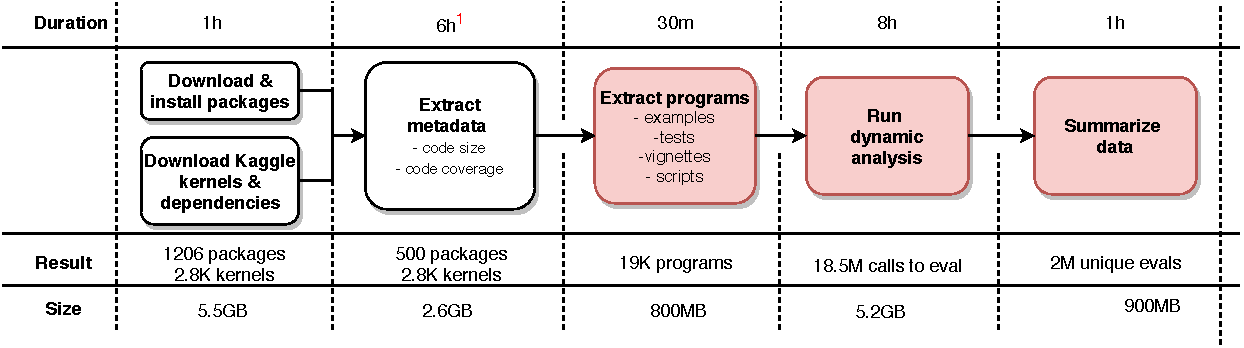
\includegraphics[width=\linewidth]
{pipeline.pdf}\caption{Pipeline}\label{fig:pipeline}
\end{figure*}

The pipeline begins with downloading and installing open source R packages from
CRAN for the corpus along with their dependencies. The Kaggle programs are
downloaded from \href{http://www.kaggle.com}{Kaggle} separately by a crawler.
Next, code size and coverage metrics from the installed packages are extracted
using the \href{ https://github.com/r-lib/covr}{\covr} package. This is followed
by extraction of runnable programs from R packages: tests, examples and
vignettes. The extracted programs are then run through \emph{evil} (\emph{Ev}al
\emph{I}nspection \emph{L}ibrary), a dynamic analyzer that collects information
about \eval calls from program runs. This dynamic analyzer builds upon our
dynamic analysis framework, \instrumentr which is another R package that enables
us to write our dynamic analysis logic in R. It internally uses a modified R
interpreter, \rdyntrace~\cite{oopsla19a}, that exposes hooks from within the
interpreter implementation for events of interest. \instrumentr serves as an
intermediary between \rdyntrace and \evil, it intercepts the hooks exposed by
\rdyntrace and attaches R functions exported by \evil as callbacks. The \evil
callbacks execute on corresponding interpreter events. All steps of this
pipeline are parallelized. To schedule and parallelize extraction and analysis
of programs, we use our homegrown library \runr. Furthermore, \runr gracefully
handles and reports failures across large-scale program runs which greatly aids
debugging of the analysis pipeline. The data extracted by \evil from each
program is concatenated, cleaned and summarized in the post-processing phase by
custom R scripts. Finally, the summarized data is analyzed in RMarkdown
notebooks to gather insights. Apart from the figures, the data points included
in the paper are also generated by RMarkdown notebooks as latex macros.

\section{Corpus}

In this study, we report on \eval usage in a corpus of \CorpusCorePackages R core
and \CorpusPackages popular CRAN packages. To quantify the eval use, we run
\CorpusAllProgramsRnd of R programs that are extracted form those packages as
well as from the user-written data-analyses shared on the Kaggle platform. In
this section we describe this corpus and methodology used to assemble it.

\subsection{CRAN Packages}

We have selected the TOP \CorpusPackages packages based on the number of reverse
dependencies, \ie how many other packages depend on them\footnote{Extracted from
  package metadata using builtin function}. Using this criterion helps us to
choose popular packages which in general should be of a better quality and have
better code coverage and therefore more code to run. The resulting set has
\summary{CorpusRevdeps}\footnote{Such triples represent ($min$ / $mean$ /
  $max$)} reverse dependencies and consists of \CorpusRCodeRnd lines of R code
and \CorpusNativeCodeRnd lines of native code (C/C++/Fortran)\footnote{Excluding
  comments and blank lines using \url{github.com/AlDanial/cloc}}.
Figure~\ref{fig:corpus} shows these packages, the size of the dots reflects the
project's size in lines of code including both R and native code, the x-axis
indicates the expression code coverage in percents and the y-axis gives the
number of reverse dependencies in log scale. Dotted lines indicate means.
Packages with over \CorpusEvalsPackageTreshold eval call sites are annotated.

\begin{figure*}[!tb]\centering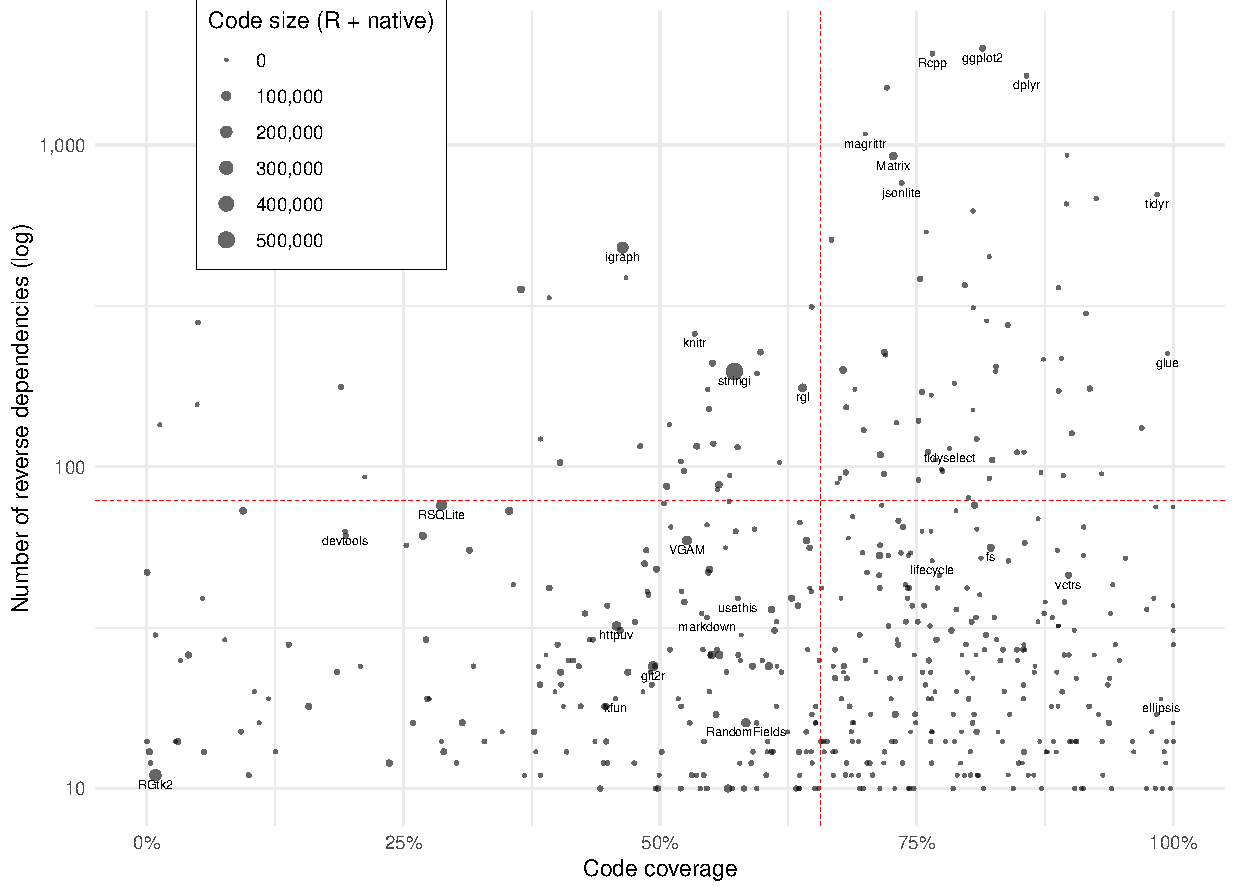
\includegraphics[width=\linewidth]
  {corpus.pdf}\caption{CRAN packages}\label{fig:corpus}
\end{figure*}

All included packages come from the Comprehensive R Archive Network
(CRAN\footnote{\url{http://cran.r-project.org}}), the largest repository of R
code with over \CorpusAllCranRnd packages\footnote{CRAN receives about 6 new
  package submissions a day~\cite{Ligges2017}}. Unlike other open code
repositories such as GitHub, CRAN is a curated repository. Each submitted
package must abide to a number of well-formedness rules that are automatically
checked asserting certain quality. Most relevant for this work is that all of
the \emph{runnable code} is tested and only a successfully running package is
admitted in the archive. This is important as we use this runnable code for the
dynamic analysis of eval calls.

There are three sources of runnable code in a R package. Next to the package
\emph{tests}, there are also \emph{examples} and \emph{vignettes}. Examples are
R code snippets extracted from package documentation into scripts file.
Vignettes are long-form description of package functionality written using
literate-programming style in \LaTeX\xspace or Rmarkdown with chunks of R code
that can be similarly extracted into R scripts. R provides builtin functions for
tangling the embedded code into files.

The selected packages contain \CorpusPackagePrograms programs with
\CorpusPackageProgramsCodeRnd lines of R code:
%
\begin{compactitem}[$-$]
  \item \CorpusExamplesProgramsRnd examples with \CorpusExamplesCodeRnd
  \summaryrnd{CorpusExamplesCode} lines of code,
  \item \CorpusTestsProgramsRnd tests with \CorpusTestsCodeRnd
  \summaryrnd{CorpusTestsCode} lines of code, and
  \item \CorpusVignettesProgramsRnd vignettes with \CorpusVignettesCodeRnd
  \summaryrnd{CorpusVignettesCode} lines of code.
\end{compactitem}

For each package we use its runnable code to compute the package code
coverage\footnote{Computed using \url{ https://github.com/r-lib/covr}}. On
average, across the \CorpusPackages packages, it is \CorpusMeanExprCoverage.

\subsection{Kaggle Scripts}

To represent user-written code in the corpus, we turned to
Kaggle\footnote{\url{https://www.kaggle.com}}, an online platform for
data-science and machine-learning practitioner. Among others, the website allow
people to share data-science competitions, a data-analysis problem together with
data, for which users try to find the best solution. The solutions, called
\emph{kernels}, are then shared back to the platform in the form of either plain
scripts or as Rmarkdown / Jupyter notebooks written in either Julia, Python, R
or SQLite.

One of the most popular competition is about predicting passenger survival on
Titanic\footnote{\url{https://www.kaggle.com/c/titanic}} with \CorpusKaggle
kernels in R (over 1/4 of all available R kernels) which we used for our corpus.

Unlike CRAN, Kaggle is not a curated repository and therefore there are no
guarantees about the quality of the code. After downloading all of the
\CorpusKaggle kernels and extracting the R code from the various
formats\footnote{We use \texttt{rmarkdown} package to convert from Jupyer
  notebook to Rmarkdown as well as to convert from Rmarkdown to plain R}, we
found that \CorpusDuplicatedKaggle were whole-file duplicates. From
\CorpusRunnableKaggle kernels, \CorpusFailedKaggle failed to execute. Next to
various runtime exceptions, common problems were parse errors and misspelled
package names.

The final set contains \CorpusFinishedKaggle kernels with
\CorpusFinishedKaggleCodeRnd \summaryrnd{CorpusFinishedKaggleCode} lines of R
code.

\subsection{Summary}

Together, we have assembled a corpus of \CorpusPackages R packages and
\CorpusFinishedKaggle user-written data-analysis scripts. Together it contains
\CorpusAllCodeRnd lines of source code (both and R and native code). Out of
this, \CorpusAllRunnbaleCode lines R code spread across \CorpusAllPrograms R
scripts is the code that we run during the dynamic analysis.

\section{Usage Metrics}

This section presents an overview of the usage of \eval in our corpus.
Previous work reported that 82\% of JavaScript-enabled web pages used
\eval~\cite{ecoop11}. The case for R is more striking with 100\% of the
programs using that \eval.\footnote{In this section, we combine calls to
  \c{eval}, \c{eval.parent}, \c{evalq} and \c{local}.}  This high number is
explained by the fact that the R implementation, its core packages, use
\eval extensively. In our analysis, we differentiate uses of \eval based on
where they originate from. A {\bf core} \eval is one that occurs in the code
of a core package.  A {\bf dependent} \eval is one that occurs in a package
that was included by the target package. An {\bf own} \eval is one that
occurs in the source code of the target package.

Over all, we observed \AllAllCallCountRnd calls to \eval in the
\CorpusAllProgramsRnd programs in our corpus.  Table~\ref{A} details this
run-time information. The format is T (m/M/x) where T is the total number of
calls observed for all runs of the corpus, m and x are the minimum and
maximum number of calls for any given run, and M is the mean number of calls
per run. We can observe that an average run of CRAN package will trigger 581
{\eval}s in core package, 532 in dependent packages and 292 in the package
itself.  The Kaggle data set has small programs, and, these programs only
trigger \eval in core and dependent packages. Thus, an average Kaggle run
has 412 core calls, 96 dependent calls, and no own calls.


\begin{table}[ht]
\resizebox{\columnwidth}{!}{%
\begin{tabular}{@{}r|ccc@{}} \hline
Source & Core & Dependent & Own \\\hline
      %      CRAN & \CranCoreTotalEvalCallsRnd (\CranCoreMinEvalCallsRnd/\CranCoreAvgEvalCallsRnd/\CranCoreMaxEvalCallsRnd) & \CranDependentTotalEvalCallsRnd (\CranDependentMinEvalCallsRnd/\CranDependentAvgEvalCallsRnd/\CranDependentMaxEvalCallsRnd) & \CranOwnTotalEvalCallsRnd (\CranOwnMinEvalCallsRnd/\CranOwnAvgEvalCallsRnd/\CranOwnMaxEvalCallsRnd) \\
CRAN & \CranCoreTotalEvalCallsRnd (1 / 581 / 416K)  & \CranDependentTotalEvalCallsRnd (1 / 532 / 183K) & \CranOwnTotalEvalCallsRnd (1 / 292 / 144K)\\
Kaggle & \KaggleCoreTotalEvalCallsRnd (1 / 412 / 2.8K) & \KaggleDependentTotalEvalCallsRnd (3 / 96 / 1.1K) & 0 (0 / 0 / 0) \\
%      Kaggle & \KaggleCoreTotalEvalCallsRnd (\KaggleCoreMinEvalCallsRnd/\KaggleCoreAvgEvalCallsRnd/\KaggleCoreMaxEvalCallsRnd) & \KaggleDependentTotalEvalCallsRnd (\KaggleDependentMinEvalCallsRnd/\KaggleDependentAvgEvalCallsRnd/\KaggleDependentMaxEvalCallsRnd) & 0(0/0/0) \\
      \hline
    \end{tabular}
  }
  \caption{Eval calls in CRAN and Kaggle}
  \label{A}
\end{table}



%% The following table will be replaced. {\bf <At this point separating between
%%   the different kinds of evals is distracting. We have not argued why it is
%%   important.>}

%% \begin{table}[ht]\resizebox{\columnwidth}{!}{\begin{tabular}{l|rr|r||rr|r}\hline
%% \multicolumn{1}{c}{Function}& \multicolumn{3}{c}{Calls} & \multicolumn{3}{c}{Callsites}\\
%% \cline{1-1} \cline{2-4} \cline{5-7}
%% & Core & Packages & Total & Core & Packages & Total\\\hline
%% \c{eval} & \CoreEvalCallCountRnd & \PackageEvalCallCountRnd  & \AllEvalCallCountRnd & \CoreEvalSiteCountRnd & \PackageEvalSiteCountRnd &  \AllEvalSiteCountRnd\\
%% \c{eval.parent} & \CoreEvalParentCallCountRnd & \PackageEvalParentCallCountRnd  & \AllEvalParentCallCountRnd & \CoreEvalParentSiteCountRnd & \PackageEvalParentSiteCountRnd & \AllEvalParentSiteCountRnd\\
%% \c{evalq} & \CoreEvalqCallCountRnd & \PackageEvalqCallCountRnd  & \AllEvalqCallCountRnd & \CoreEvalqSiteCountRnd & \PackageEvalqSiteCountRnd & \AllEvalqSiteCountRnd \\
%% \c{local} & \CoreLocalCallCountRnd & \PackageLocalCallCountRnd  & \AllLocalCallCountRnd & \CoreLocalSiteCountRnd & \PackageLocalSiteCountRnd & \AllLocalSiteCountRnd \\\hline
%% Total & \CoreAllCallCountRnd & \PackageAllCallCountRnd  & \AllAllCallCountRnd & \CoreAllSiteCountRnd & \PackageAllSiteCountRnd & \AllAllSiteCountRnd \\  \hline
%% \end{tabular} } \label{table:eval-count-summary}
%%  \caption{Distribution of eval calls and callsites in the corpus}
%% \end{table}

%% \ref{table:top-ten-package-summary} shows the number of calls to eval
%% made by the ten most frequent callers to eval. These packages together have
%% \missingNumber callsites and account for \missingPercentage calls to eval.
%% Furthermore, the top ten callsites account for \missingPercentage of package
%% eval calls. A single callsite of \TopTenPackageNameA accounts for over
%% \missingPercentage calls to eval.

%% \begin{table}[ht]
%%   \resizebox{\columnwidth}{!}{%
%%     \begin{tabular}{l|rrr||l|rrr}
%%       \hline
%%       \multicolumn{4}{c}{}& \multicolumn{4}{c}{} \\
%%       \cline{1-4} \cline{5-8}
%%       Package & Callsites & Calls & Calls \% & Package & Callsites & Calls & Calls \%\\
%%       \hline
%%       \TopTenPackageNameA & \TopTenPackageCallsiteCountA & \TopTenPackageCallCountA &\TopTenPackageCallPercA & \TopTenPackageNameF & \TopTenPackageCallsiteCountF & \TopTenPackageCallCountF & \TopTenPackageCallPercF \\
%%       \TopTenPackageNameB & \TopTenPackageCallsiteCountB & \TopTenPackageCallCountB &\TopTenPackageCallPercB & \TopTenPackageNameG & \TopTenPackageCallsiteCountG & \TopTenPackageCallCountG & \TopTenPackageCallPercG \\
%%       \TopTenPackageNameC & \TopTenPackageCallsiteCountC & \TopTenPackageCallCountC &\TopTenPackageCallPercC & \TopTenPackageNameH & \TopTenPackageCallsiteCountH & \TopTenPackageCallCountH & \TopTenPackageCallPercH \\
%%       \TopTenPackageNameD & \TopTenPackageCallsiteCountD & \TopTenPackageCallCountD &\TopTenPackageCallPercD & \TopTenPackageNameI & \TopTenPackageCallsiteCountI & \TopTenPackageCallCountI & \TopTenPackageCallPercI \\
%%       \TopTenPackageNameE & \TopTenPackageCallsiteCountE & \TopTenPackageCallCountE &\TopTenPackageCallPercE & \TopTenPackageNameJ & \TopTenPackageCallsiteCountJ & \TopTenPackageCallCountJ & \TopTenPackageCallPercJ \\
%%       \hline
%%     \end{tabular}
%%   }
%%   \label{table:top-ten-package-summary}
%%   \caption{Distribution of eval calls and callsites in the top ten packages}
%% \end{table}


Table \ref{table:site-package-summary} shows the results of static analysis
for the CRAN packages in our corpus. 89 packages have a single call site,
and one package has \miss{252} call sites of \eval. \miss{XXX} packages have
no calls to \eval. The core packages have \miss{41} callsites of eval and
Kaggle has none. These static numbers are under approximations as \eval may
be called reflectively, through aliases, or passed to a higher-order function.

\begin{table}[ht]\resizebox{\columnwidth}{!}{%
\begin{tabular}{rr|rr|rr}\hline
Callsites & Packages & Callsites & Packages & Callsites & Packages \\ \hline
\SiteSummarySiteCountA & \SiteSummaryPackageCountA & \SiteSummarySiteCountF & \SiteSummaryPackageCountF & \SiteSummarySiteCountK & \SiteSummaryPackageCountK \\
\SiteSummarySiteCountB & \SiteSummaryPackageCountB & \SiteSummarySiteCountG & \SiteSummaryPackageCountG & \SiteSummarySiteCountL & \SiteSummaryPackageCountL \\
\SiteSummarySiteCountC & \SiteSummaryPackageCountC & \SiteSummarySiteCountH & \SiteSummaryPackageCountH & \SiteSummarySiteCountM & \SiteSummaryPackageCountM \\
\SiteSummarySiteCountD & \SiteSummaryPackageCountD & \SiteSummarySiteCountI & \SiteSummaryPackageCountI & \SiteSummarySiteCountN & \SiteSummaryPackageCountN \\
      \SiteSummarySiteCountE & \SiteSummaryPackageCountE & \SiteSummarySiteCountJ & \SiteSummaryPackageCountJ & \SiteSummarySiteCountO & \SiteSummaryPackageCountO \\    \hline
\end{tabular}} \label{table:site-package-summary}
\caption{Distribution of callsites in CRAN}
\end{table}


To roughly estimate the complexity of the code being evaluated,
Fig.~\ref{fig:ast-size} shows the distribution of the abstract syntax tree
size of the \c{expr} argument to \eval. The majority of inputs across core
and packages (\miss{XX}\%) is 1. That is to say, the code being evaluated
consists of a single variable name or constant. A function call needs at
least three nodes. Inputs smaller than \c{X} nodes account for 95\% of all
calls. Sizes are roughly similar between core and packages.

\begin{figure}[htbp]
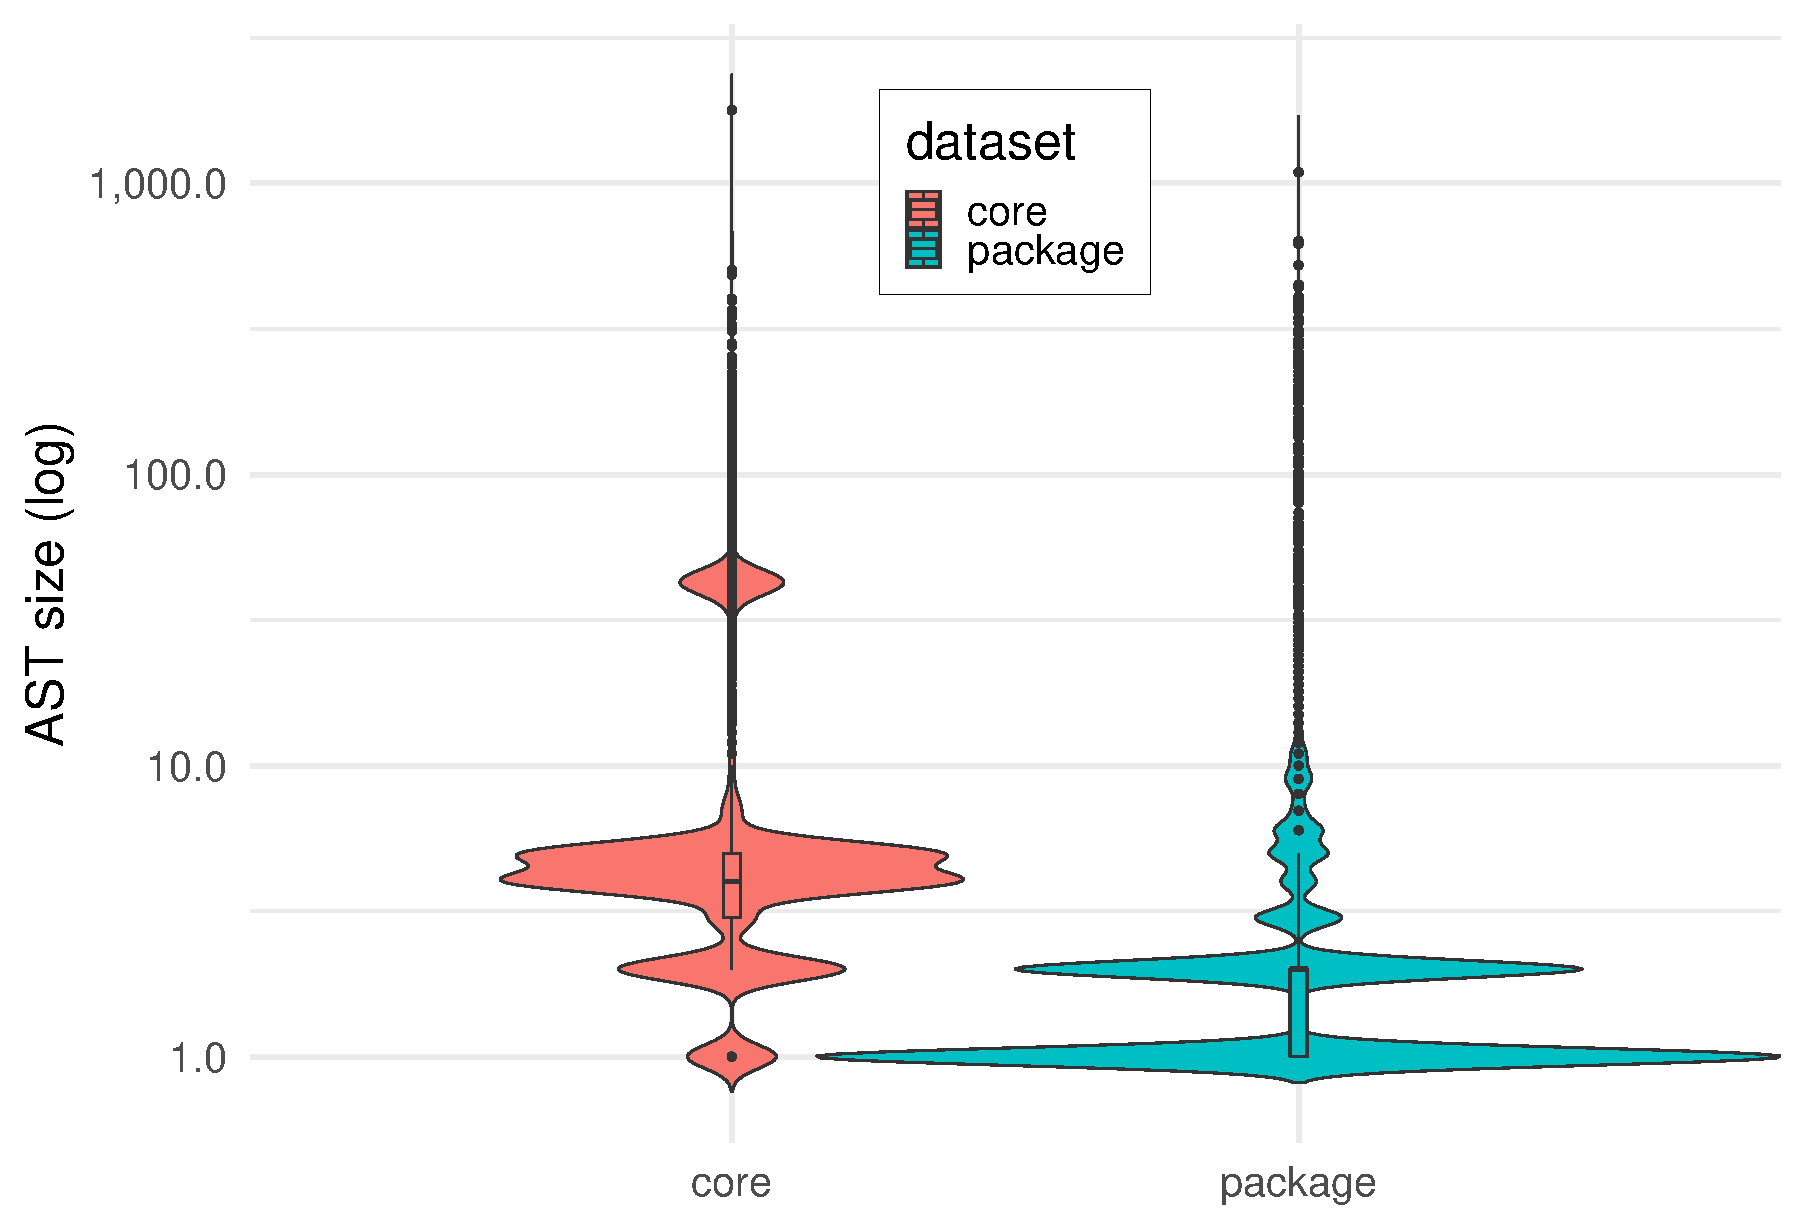
\includegraphics[width=\columnwidth]{ast_sizes}
\caption{Input sizes} \label{fig:ast-size}
\end{figure}

\medskip\noindent\emph{Discussion:} Comparing the use of \eval in R and
JavaScript is instructive. The use of \eval is more widespread in data
science code than it was in JavaScript. Any run of an R program seems to
trigger \eval, more over package programmers use \eval liberally. On the
other hand, the authors of Kaggle packages do not use the feature at all.
This point to a bifurcated user community, experts who write package know
how to use \eval while end-users do not. An alternative explanation is that
end-users do not need \eval for simple data analysis tasks. This bifurcation
was not observed in the JavaScript community, but this may have changed with
the advent of Node.js ecosystem.  The distribution of input sizes is similar
to that found in JavaScript, the majority of inputs being rather small.


{\bf Missing from this section is the measure of the number of events
  happening in an eval}

\section{A taxonomy of eval}

We first classify \c{eval} depending on the resolved expression, \emph{i.e.}
the first argument of \c{eval} after all possible function calls and symbol
resolution in it have been executed.

\subsection{Operation mix}

Here we should show some information about what happens during an eval. What kinds of operations...



\subsection{Scope}

Here we talk about scopes and envs

One of the main differences of the R \eval with the javascript one is how it
interacts with \emph{scope}, or environments in R. In Javascript, \c{eval}
can access the local scope and the global scope. In R, \c{eval} has an
argument \c{envir} to indicate in which environment its first argument,
after being resolved, must be evaluated. By default, it is equal to \c{parent.frame()}, which is the parent environment of the \c{eval} call.

 This argument can also be \c{NULL}, a list or a dataframe. In that case, \c{eval} copies \c{envir} and encloses it the environment defined by \c{enclos}. Finally, the argument can also be a number $n$. It means that the environment in which the expressions is evaluated will be the results of \c{sys.call(n)} where $n$ refers to the $n$-th call frame after the global environment.

\textbf{Do we speak more about what an environment is, \c{.GlobalEnv}, \c{emptyenv()}, environment navigation here, or in the Background section?}

We classify the environment from two points of view:
\begin{itemize}
	\item in which environment \c{eval} writes new bindings 
	\item in which \emph{existing} environment \c{eval} reads. It is the first non new environment. \c{eval} will also be able to read in all parent environment of that environment. 
\end{itemize}

% Variability: how many different envir class, and different envir expr, for one call site?

\subsection{Patterns}

This section presents the common patterns of \eval usage in our corpus. We
randomly selected 20 packages from the corpus and studied how they use eval.
We have grouped those uses in the following categories.

  \subsubsection{Evaluation using Data Fields} A common use of \eval is to
  evaluate expressions that access data frame columns or list (heterogeneous
  vectors) elements by name. Core R provides two functions, \c{with} and
  \c{within} that implement this pattern. These functions construct a temporary
  environment with data frame columns or list elements as the bindings.
  Side-effects performed by the evaluated expression take place in this temporary
  environment and are ignored by the \c{with} function. The \c{within} function
  copies these modifications to a local copy of the input data and returns it.
  This pattern is used quite often for statistical modeling. The modeling
  expressions is constructed from variable names whose values are supplied by a
  data frame or list.

  \subsubsection{Sandboxing} The combination of \eval and first class
  environments can be used to construct a sandbox for evaluating side-effecting
  expressions. The newly constructed environment can use the current environment
  for its lexical scope. This provides the evaluated expression access to all the
  bindings in the current scope but restricts the side-effect to the newly
  constructed throwaway environment. However, this sandboxing is limited because
  the expression can reflectively access any environment in the call stack or use
  the super assignment operator(\c{<<-}) to write to parent scope. The \c{local}
  function which is part of Core R is an example of this usage pattern.

  \subsubsection{Dynamic Code Loading} The combination of \parse and \eval is
  used to parse text from string or file and evaluate in a custom environment.
  This pattern is used by the \source Core R function to load R code from a file
  in the current workspace. This is quite useful for loading functions for
  interactive data analysis.

  \subsubsection{Metaprogramming} The combination of \eval and \substitute is
  used to do metaprogramming in R. \substitute can be used to synthesize ASTs by
  stitching together user inputs. \substitute walks over its argument AST and
  replaces the symbols with their bindings in the specified environment and
  returns this new AST which can then be evaluated in custom environments using
  \eval.

  \subsubsection{Convenience}
  evaling recorded calls in model-fitting functions or passing most of the
  current call to another function. Both ``patterns'' use the \c{match.call} to
  capture current call. The latter is just for laziness as it is the same as
  calling the new function with explicitly selecting the arguments.

  \subsubsection{Miscellaneous} \eval is also used in R packages to get around
  various limitations. For example, in \datatable package, \eval is used to modify
  a binding in the \base package of R. Bindings in the \base package are locked
  for modification and require explicit unlocking using \unlockBinding function.
  However, directly using this function triggers a warning during package building
  process which statically analyzes the package for use of such restricted
  functions. The \datatable gets around this limitation by enclosing the call to
  \unlockBinding inside \eval.

\subsection{Provenance}

Here we talk about where the input of an eval comes from.

Although \c{eval} takes an R expression, it can evaluate a string if this string is first parsed with \c{parse}, \c{str2expression} or \c{str2lang}. This happens for \PercentParsedEvals of the eval calls, and \PercentParsedCallSites of the call sites.

This corresponds to strings loaded from a file or to metaprogramming, \ie building new variables or functions by concatenating strings together, as in Listing~\ref{code:parsepaste}. To detect this kind of metaprogramming, we look at the usage of the main concatenating functions in R, \c{paste}, \c{paste0}, \c{glue} and \c{str_c}, and \PasteParsedEvals of the evals and \PasteParsedCallSite of the call sites using a parse function actually call a concatenating function.


\begin{lstlisting}[caption={Using \c{eval} and \c{parse} to do meta-programming in package \emph{data.table}, to build the options at load time (in \emph{onLoad.R}).}, label=code:parsepaste]
eval(parse(text=paste0("options(",i,"=",opts[i],")")))
\end{lstlisting}

\textbf{What about a table of packages ranked by usage of parse (and/or paste...)?}


\subsection{Consistency}

Here we talk about whether the same call site sees the same pattern

{\bf Polymorphic may not be the right word.}

We look at how \emph{polymorphic} the \c{expr} argument of \eval can be, \ie
how many different types of the resolved \c{expr} there are per call sites,
in Figure~\ref{fig:polymorphism}. \PercentMonomorphic of the call sites are
\emph{monomorphic}.

\begin{figure}[!h]
    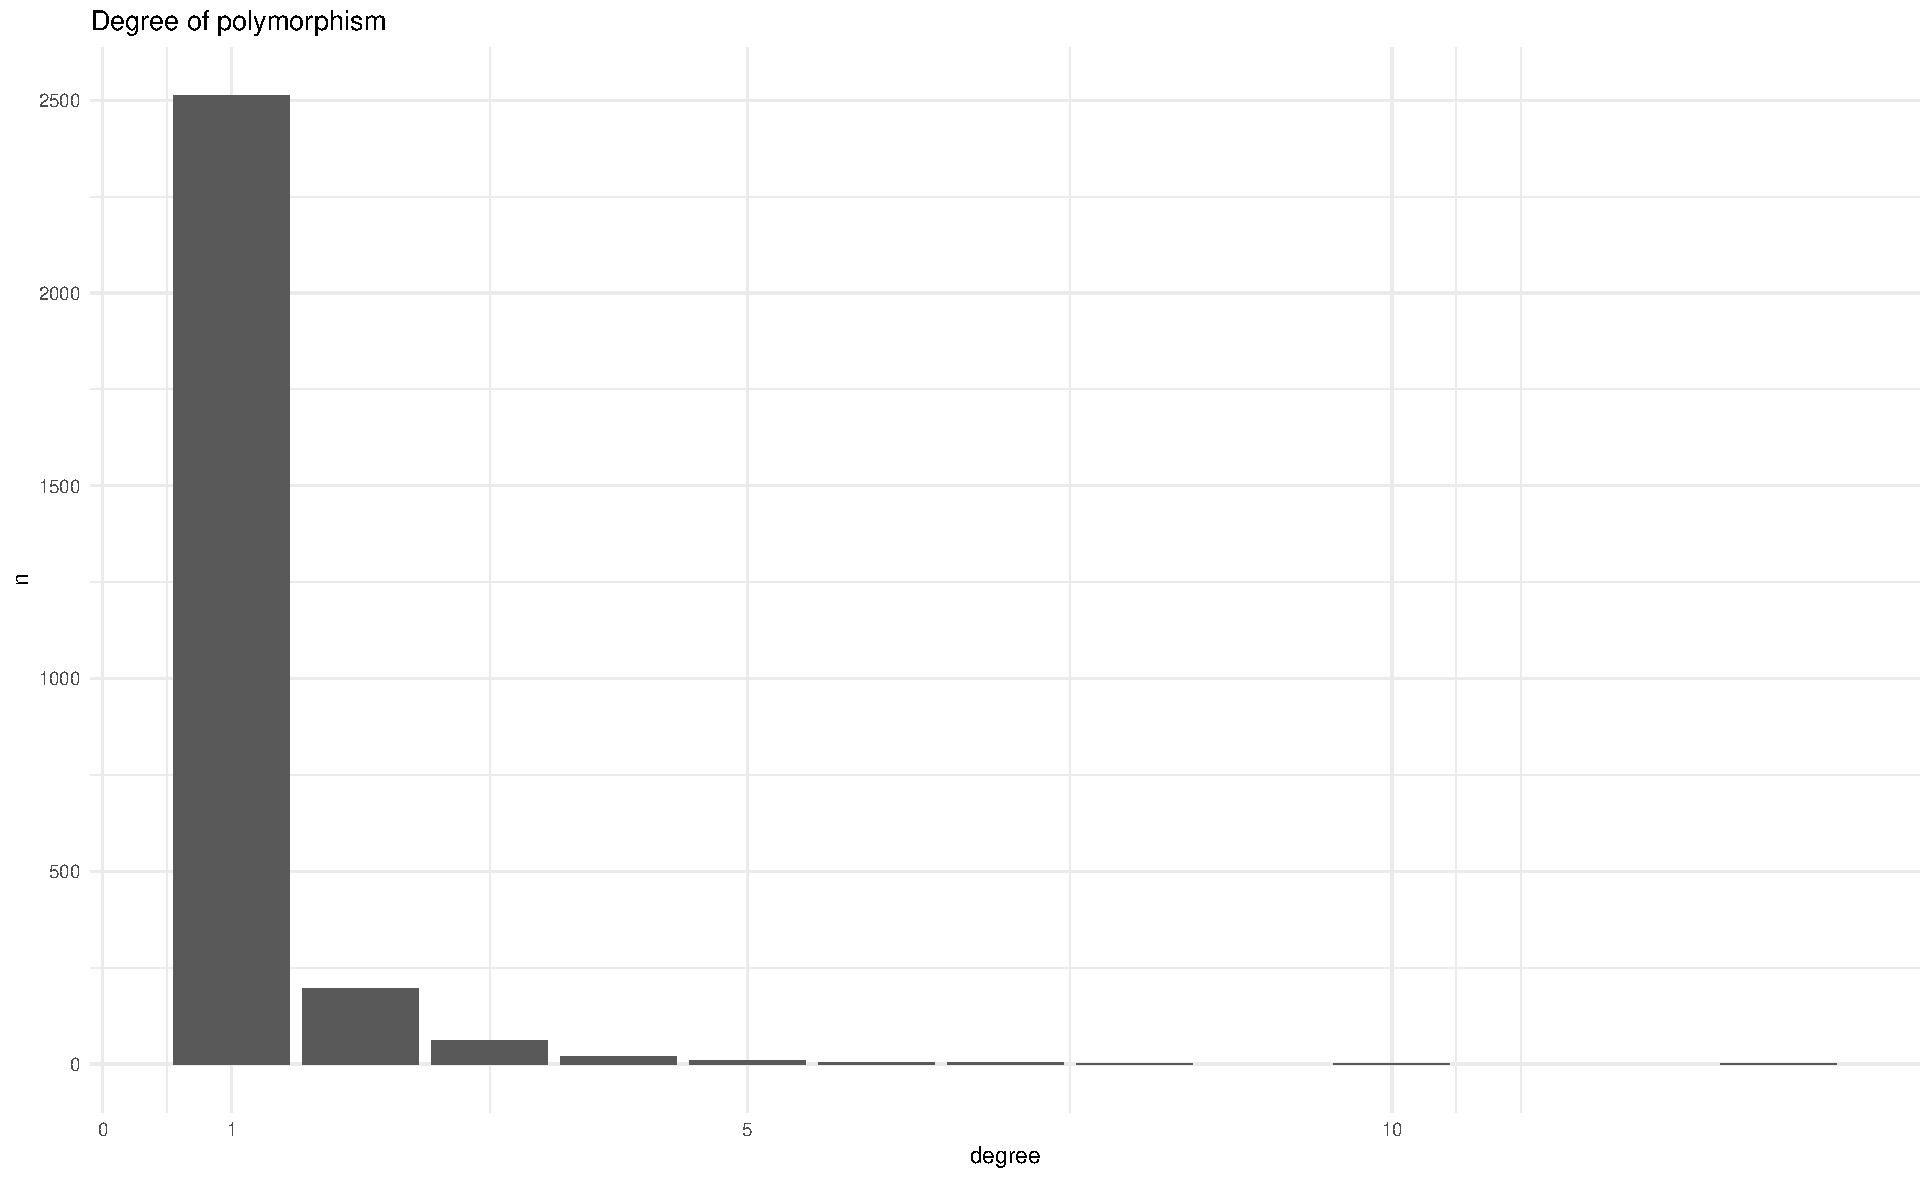
\includegraphics[width=\columnwidth]{polymorphism}
    \caption{Degree of polymorphism of \c{expr} per call sites.} \label{fig:polymorphism}
\end{figure}

\subsection{base}

There are 30 functions in \emph{base} that use \eval. Only five of them use \c{parse}, for legitimate reasons, such \c{source} and \c{sys.source} which load a file and then evaluate it, or \c{invokeRestartInteractively} which prompts the user for arguments to restart execution after an error.

We endeavored  to write these functions without \eval. \c{match.arg} appears in \MatchArgPercent of the \eval calls. It is used to get the arguments, possibly abbreviated, of a function. With one argument, as \c{match.arg(arg)}, it uses \c{eval} to infer them from a parent function's formal arguments. We can rewrite it using its version with two arguments, \c{match.arg(arg, choices)} where \c{choices} are the possible formal arguments of the function, as shown in Listing~\ref{code:matcharg}.

\begin{lstlisting}[caption={Rewriting \c{match.arg} without \eval}, label=code:matcharg]
f <- function(type=c("examples", "tests", "vignettes")) {
actual_type = match.arg(type)
...
}

f <- function(type=c("examples", "tests", "vignettes")) {
actual_type = match.arg(type, choices=c("examples", "tests", "vignettes"))
...
}
\end{lstlisting}

\section{Threats to Validity} The primary threat to validity is the issue of
code coverage, a cause of concern for any dynamic approach. We mitigate this by
including only those R packages in our corpus that have many reverse
dependencies and thus high code coverage. Secondly, we turn off the bytecode
compiler for this study. The bytecode compiler can also call eval. Thirdly, we
do not get source locations for \UndefinedEvalsRnd eval calls. In these cases
\eval is either passed as an argument to a higher-order functions or is defined
in a function returned by a higher-order function and the R parser does not
retain location information for \eval. However, this is a meager
\PercentUndefinedEval of all eval calls and is unlikely to affect our analysis.

\section{Conclusion}

\bibliographystyle{IEEEtran}
\bibliography{bib/bibliography,bib/jv}

\end{document}
